% abstract_takada.tex
% #################################################

\documentclass{article_vdlab_sotsuron_youshi}
\pagestyle{empty}

\usepackage{setspace}
\usepackage{graphicx}
\usepackage{amsmath,amssymb}
\usepackage{comment}
\usepackage{here}

%2段組みの段組み間間隔を設定
\columnsep=1.5cm

\begin{document}
%文字間隔の設定
\kanjiskip = .7pt plus3pt minus 3pt
\xkanjiskip = .7pt plus 3pt minus 3pt
\small
\setstretch{1.1}

%図回りの余白を設定
\setlength{\abovecaptionskip}{0mm}
\setlength{\belowcaptionskip}{0mm}
\setlength{\floatsep}{0mm}
\setlength{\textfloatsep}{0mm}
\setlength{\intextsep}{3mm}
\setlength{\dblfloatsep}{0mm}
\setlength{\dbltextfloatsep}{0mm}

% #################################################

\twocolumn[
  \begin{center}
    % 論文題目と氏名
    \jtitle{HILSにおけるアクチュエータの制御手法の検討}
    \jauthors{田中 隆之}
    \etitle{Study on Actuator Control Method with Hardware-in-the-Loop Simulation System}
    \eauthors{Takayuki Tanaka}
  \end{center}
]

%文字間隔の設定
\kanjiskip = .7pt plus3pt minus 3pt
\xkanjiskip = .7pt plus 3pt minus 3pt
\small
\setstretch{1.1}

% #################################################
\section{緒言}
車両開発において,シミュレーションや実車走行試験による車両運動性能の評価が行われている.
シミュレーションによる評価は,路面状況や天候などの影響を受けずに同一条件での試験が可能である.また,実車走行試験では,ハードウェアの非線形特性を考慮した評価が可能である.これらを組み合わせた評価手法として,Hardware-in-the-Loop Simulation ( 以下HILS )がある.HILSシステムは評価対象の一部をハードウェアとしてシミュレーションのループ内に組込み特性を評価する手法であり,開発期間の短縮や品質の向上に寄与する重要なツールとなっている\cite{1}.HILSシステムはハードウェアの計測結果を含む解析モデルの計算結果に基づいてアクチュエータを制御し特性評価を行うシステムである.\par
本研究では,自動車のタイヤ-サスペンション系の上下動を再現するHILSシステムを対象として,アクチュエータの制御手法を検討する.アクチュエータの制御手法はHILSシステムの再現性に影響を及ぼす.ハードウェアに生じる摩擦の影響を考慮した制御手法を検討した.ハードウェアの挙動とリアルタイム解析結果を比較することで,検討した制御手法におけるHILSシステムの再現性の影響を評価した.
% #################################################
\section{HILSシステム}
\subsection{HILSシステムの概要}
本研究室で開発されたHILSシステムは自動車のタイヤ-サスペンション系の上下動を試験機で再現するシステムである.HILSシステムの概要を図\ref{fig:HILS}に示す.このHILSシステムは,車両運動解析やシステム制御を行うソフトウェア部と,ハードウェアである試験装置から構成される.本システムでは試験装置のばね上-ばね下相対変位が解析結果と一致するように制御を行う.解析モデルには上下2自由度モデルを用いる.計測されたダンパの減衰力を用いて解析を行い,解析結果に基づき路面下部に設置されたアクチュエータの入力を決定することにより,上下挙動の再現が可能である.
\vspace*{3mm}
\begin{figure}[H]
  \begin{center}
    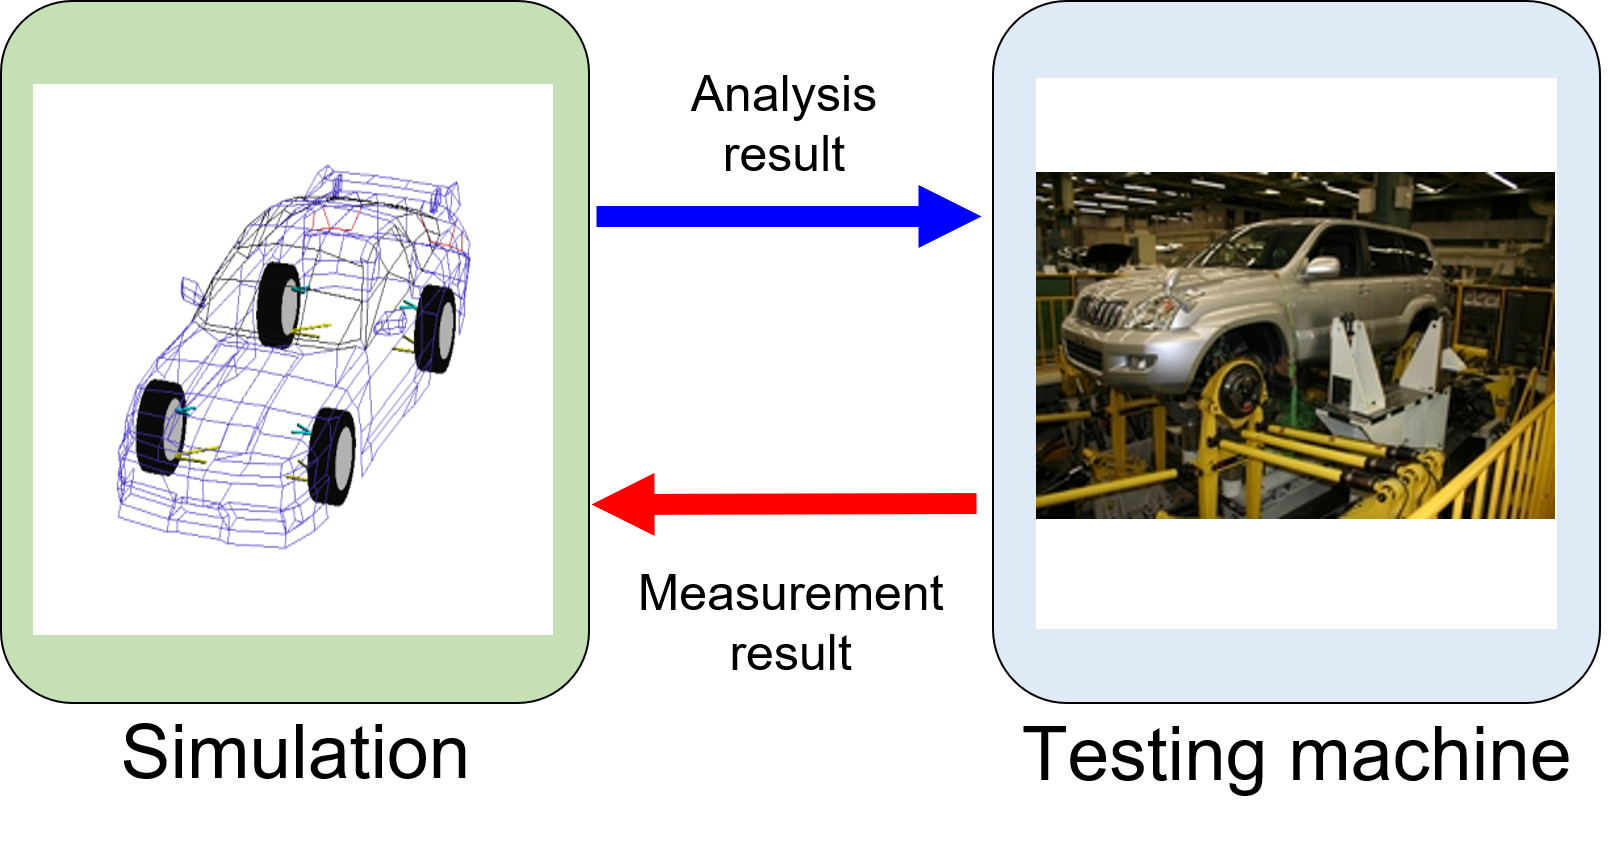
\includegraphics[height=60mm]{figure/HILS.eps}
    \vspace*{-1mm}
    \caption{System Overview of Tire-Suspension HILS System}
    \label{fig:HILS}
  \end{center}
\end{figure}
% \vspace{-2mm}
% \begin{figure}[H]
%   \centering
%    \includegraphics[height=25mm]{figure/Block_Diagram_t_r.eps}
% \caption{Block diagram(Relative)}
%   \label{fig:R}
% \end{figure}

\subsection{解析モデル}
解析モデルに用いた上下2自由度モデルは,車両の上下動を表すことのできるモデルである\cite{7}.
上下2自由度モデルを図~\ref{fig:Analysis Model}~に示す.
諸元を表~\ref{tab:parameter}~に示す.
また,このモデルの運動方程式は以下である.

\vspace*{-5mm}
\begin{flalign}
 \label{eq:1} &m_1\ddot x_1 + k_1(x_1-x_0) + k_2(x_1-x_2) - f_c = 0\\
 \label{eq:2} &m_2\ddot x_2 + k_2(x_2-x_1) + f_c = 0
\end{flalign}

\noindent
ここで,$m_1$はばね下質量 ,$m_2$はばね上質量,$k_1$,$k_2$はばね定数,$f_c$はダンパ力,$x_0$は路面変位,$x_1$はばね下変位,$x_2$はばね上変位である.

\begin{figure}[H]
  \begin{minipage}{0.5\hsize}
    \begin{center}
      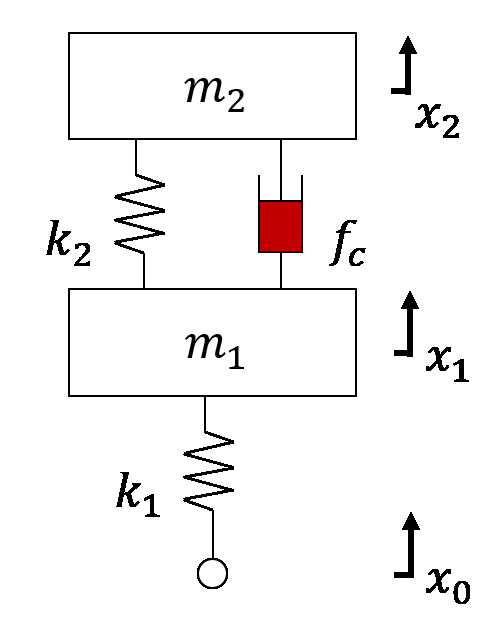
\includegraphics[height=30mm]{figure/analysis_model.eps}
      \vspace*{1mm}
      \caption{Analysis Model}
    \label{fig:Analysis Model}
    \end{center}
  \end{minipage}
  \begin{minipage}{0.35\hsize}
      \begin{center}
	\makeatletter
	\def\@captype{table}
	\makeatother
	\caption{Parameter}
	\label{tab:parameter}
	  \begin{tabular}{cc}\hline
	    $m_1$ [kg] & 1.3\\
	    $m_2$ [kg] & 6.9\\
	    $k_1$ [N/m] & 2200\\
	    $k_2$ [N/m] & 439\\\hline
	  \end{tabular}
      \end{center}
  \end{minipage}
\end{figure}

\subsection{試験機}
HILS試験機を図~\ref{fig:testing_machine}に示す.
この装置は上下1自由度で路面部にアクチュエータを取り付けている.
アクチュエータはリアルタイム解析の結果に基づいて制御する.
タイヤ-サスペンション系をばね下とばね,ダンパで表現している.
ソフトウェア部で計算したサスペンションストロークをばね上ばね下間の変位として実現している.
また,レーザ変位計とロードセルを用いて,サスペンションストロークとダンパ力を計測している.

\vspace{5mm}
\begin{figure}[H]
 \centering
 \includegraphics[height=50mm]{figure/HILS_machine_T.eps}
 \vspace{-2mm}
  \caption{HILS Testing machine}
 \label{fig:testing_machine}
\end{figure}

% \vspace{-1mm}
% \begin{figure}[H]
%  \centering
%  \includegraphics[height=25mm]{figure/friction.eps}
%  \vspace{-2mm}
%   \caption{Mechanism to give friction}
%  \label{fig:testing_machine_f}
% \end{figure}

% **************************************************
\newpage
 \section{摩擦の影響を考慮した制御手法}
 \subsection{摩擦力の影響}
 試験機には摩擦が存在しており,HILSシステムの再現性に影響を与える.本研究ではHILSシステムにおける摩擦の影響を評価するために,試験機の摩擦の強さを変えて,路面入力試験を行った.周波数3.0Hz,振幅5mmの正弦波を入力した際の試験結果を図~\ref{fig:friction}~に示す.
 図~\ref{fig:friction}(b)のように摩擦の影響により試験機の計測結果のサスペンションストロークに変化が見られた
 \vspace{-1mm}
 \begin{figure}[h]
     \begin{tabular}{cc}
       \begin{minipage}{0.5\hsize}
 	\centering
 	  \includegraphics[height=30mm]{figure/5_3.eps}
 	  \begin{center}
 	  \vspace{-4mm}
 	  \ (A) Week friction\
 	  \end{center}
 	\end{minipage}
        \begin{minipage}{0.5\hsize}
 	\centering
 	  \includegraphics[height=30mm]{figure/5_3_f.eps}
 	  \begin{center}
 	  \vspace{-4mm}
 	  \ (B) Strong friction\
 	  \end{center}
       \end{minipage}
     \end{tabular}
     \vspace{-1mm}
     \caption{Suspension stroke}
     \label{fig:friction}
 \end{figure}
 \subsection{等価粘性減衰係数を用いた摩擦力の考慮}
 \par
 摩擦を解析で考慮する場合,摩擦によるエネルギ損失を等価な粘性減衰として置き換える手法がある.この時,設定される等価粘性減衰係数$c_f$は同一の振動系において振幅や周波数などの振動の条件によって適値が変化してしまうが,適切に設定することで摩擦を解析で容易に行うことができる.そこで本研究では解析モデルで計算されたストローク速度$(\dot{x}_1-\dot{x}_2)$と等価粘性減衰係数$c_f$をかけることで摩擦力を粘性減衰$f_f$として解析モデル内に考慮した.摩擦力を考慮した解析モデルを図~\ref{fig:analysis_model_GD}~に示す.また運動方程式は以下である.

 \vspace*{-3mm}
 \begin{flalign}
  \label{eq:1_f} &m_1\ddot x_1 + k_1(x_1-x_0) + k_2(x_1-x_2) - f_c - f_f= 0\\
  \label{eq:2_f} &m_2\ddot x_2 + k_2(x_2-x_1) + f_c + f_f = 0
 \end{flalign}

 \begin{figure}[H]
    \begin{center}
      \includegraphics[height=40mm]{figure/model_GD.eps}
      \caption{Analysis Model include viscous attenuation}
      \label{fig:analysis_model_GD}
    \end{center}
  \end{figure}
  \par
  \subsection{等価粘性減衰係数の適応同定}
  等価粘性減衰係数$c_f$は試験機の挙動に応じて変化する.適応同定を行うために評価関数$J$を設計した.評価関数$J$を式(\ref{eq:reptation})に示す.評価関数$J$は試験機の計測結果とリアルタイム解析の差を表現している.試験機とリアルタイム解析の差を小さくするような等価粘性減衰係数$c_f$を適応的に算出する.
   \vspace{-2mm}
   \begin{flalign}
   \label{eq:reptation} J^{n}=\frac{1}{2}\ \{w_v(\dot{x}^{n}_H-\dot{x}^{n}_M)^2 + w_d(x^{n}_H-x^{n}_M)^2 + w_c(c^{n}_f - c^{n-1}_f)^2\}
  \end{flalign}
  ここで$x_H$,$x_M$~は試験機およびリアルタイム解析のサスペンションストローク,$w_v$は試験機とリアルタイム解析のサスペンションストローク速度差に対する重みづけ係数,$w_d$は試験機とリアルタイム解析のサスペンションストローク差に対する重みづけ係数,$w_c$は等価粘性減衰係数の変化量に対する重みづけ係数である.
  \par
  等価粘性減衰係数$c_f$を適応的に算出する方法として,再急降下法を使用した.再急降下法とは関数の最小化を模索するアルゴリズムの一つである\cite{9}.評価関数$J$を等価粘性減衰係数$c_f$の関数として初期値を基に式(\ref{eq:steep})を反復計算することで等価粘性減衰係数$c_f$の値を更新していく.
  \vspace{-2mm}
  \begin{flalign}
    \label{eq:steep} c_f^{(n+1)} = c_f^{(n)} - \gamma \cdotp \frac{\partial J}{\partial c_f}
  \end{flalign}
  また$\gamma$は収束速度に関わるパラメータである.$\gamma$は大きすぎると発散する可能性があり,小さいと収束が遅くなる.
  \section{HILS試験}
  等価粘性減衰係数$c_f$を適応的に算出し,摩擦力を考慮した制御手法のHILSシステムの再現性の影響を評価を行う.周波数3.0Hz,振幅5mmの正弦波の路面入力試験を行った際の試験結果を図~\ref{fig:HILS_test}~に示す.図~\ref{fig:HILS_test}~(A)より等価粘性減衰係数$c_f$が調整されていくにつれて図~\ref{fig:HILS_test}~(B)評価関数$J$が小さくなることが確認できる.これは,試験機の計測結果とリアルタイム解析の結果の差が小さくなり等価粘性減衰係数が適応的に同定したためであると考えられる.図~\ref{fig:HILS_test}~(C)は試験開始から4秒後のサスペンションストロークであり,図~\ref{fig:HILS_test}~(D)は74秒後のサスペンションストロークである.図~\ref{fig:HILS_test}~(D)は等価減衰係数$c_f$が適応的に同定された後なので図~\ref{fig:HILS_test}~(C)と比較すると,試験機と解析モデルのサスペンションストローク差が減少していることが確認できる.
  \vspace{-1mm}
  \begin{figure}[h]
      \begin{tabular}{cc}
        \begin{minipage}{0.5\hsize}
          \centering
          \includegraphics[height=30mm]{figure/c_f.eps}
          \begin{center}
            \vspace{-4mm}
            \ (A) Equivalent damping confficient\
          \end{center}
        \end{minipage}
        \begin{minipage}{0.5\hsize}
          \centering
          \includegraphics[height=30mm]{figure/J.eps}
          \begin{center}
            \vspace{-4mm}
            \ (B)  Evacuation \par fanction\
          \end{center}
        \end{minipage}\\
          \begin{minipage}{0.5\hsize}
            \centering
            \includegraphics[height=30mm]{figure/GD_10.eps}
            \begin{center}
              \vspace{-4mm}
              \ (C) Suspension stroke \par (4s~6s)\
            \end{center}
          \end{minipage}
          \begin{minipage}{0.5\hsize}
            \centering
            \includegraphics[height=30mm]{figure/GD_70.eps}
            \begin{center}
              \vspace{-4mm}
              \ (D) Suspension stroke \par (74s~76s)\
            \end{center}
          \end{minipage}
        \end{tabular}
        \vspace{-1mm}
      \caption{Result}
      \label{fig:HILS_test}
  \end{figure}

\section{結言}
本研究では,摩擦の影響を考慮したアクチュエータの制御手法がHILSシステムにおける再現性の影響を評価した.摩擦力を等価な粘性減衰として解析モデルに置き換え等価粘性減衰係数を再急降下法により適応的に同定した.検討した制御手法により,試験機の計測結果とリアルタイム解析の結果の差が小さくなることを確認した.

\begin{thebibliography}{9}
  \bibitem{1}石塚弘道,佐々木君章,鉄道車両用HILSシステムによる仮想走行試験環境,日本機械学会第16回交通・物流部門,大会講演論文集No. 07-51(2007),pp. 37-42
  \bibitem{7}社団法人\ 自動車技術会,自動車技術ハンドブック5設計(シャシ)編,社団法人\ 自動車技術会,(1990),p. 25
  \bibitem{9}
  宮里 義彦,システム制御工学シリーズ 10 適応制御,コロナ社,2018
\end{thebibliography}

\end{document}
